% ===========================================================================
%  Nuclear Science and Engineering - classe ufficiale ANS (style/nseJournal)
%
%  Compilare con:   ./build.sh
%  Figure:          make_figures.py -> figs/fig*.pdf ; flowchart.tex (TikZ)
%  Tabelle:         make_tables.py  -> tables.tex
%  Bibliografia:    fetch_refs.py   -> references.bib (da CrossRef)
%
%  I punti marcati  % TODO  richiedono un intervento dell'autore.
% ===========================================================================
\documentclass{style/nseJournal}

\usepackage{tikz}
\usetikzlibrary{shapes.geometric,arrows.meta,positioning,fit,backgrounds,calc}
\definecolor{serpent}{HTML}{4CAF7D}
\definecolor{fren}{HTML}{E8703A}
\definecolor{nnc}{HTML}{3B7A99}
\definecolor{ga}{HTML}{F2C14E}
\definecolor{newc}{HTML}{1F6FB2}

\begin{document}

\title{Neural Network-Assisted Genetic Optimization of the Multi-Group\\
Energy Structure for Lead-Cooled Fast Reactors}

% TODO: nomi, affiliazioni ed e-mail dell'autore di riferimento
\addAuthor{\correspondingAuthor{First Author}}{a}
\correspondingEmail{name@polito.it}
\addAuthor{Second Author}{a}
\addAuthor{Third Author}{a}

\addAffiliation{a}{Politecnico di Torino, Energy Department, NEMO Group\\
Corso Duca degli Abruzzi 24, 10129 Torino, Italy}

\addKeyword{energy group structure}
\addKeyword{genetic algorithm}
\addKeyword{neural network}
\addKeyword{lead-cooled fast reactor}
\addKeyword{energy collapsing}

\titlePage

\begin{abstract}
The multi-configuration optimization of the multi-group energy structure for
lead-cooled fast reactor simulations has been shown to depend on the random seed
of the genetic algorithm, different seeds producing different structures of
comparable quality. This behaviour indicates a rugged objective landscape, whose
characterization requires a number of independent searches far beyond what the
existing workflow can afford, since every candidate structure must be evaluated
with a full-core calculation. The present work removes that constraint by
introducing a neural metamodel of the fitness functions, trained on 91\,723
full-core evaluations of the NEA lead-cooled fast reactor benchmark performed
with the neutronics module of FRENETIC. The metamodel predicts the fifteen
fitness functions, five physical quantities for each of three control-rod
configurations, with a mean coefficient of determination of $0.99634$ and a
median relative error of $0.403\%$ on an external validation set, and evaluates
a candidate structure several orders of magnitude faster than the solver. One
hundred independent searches are then completed in $79$~s, and the resulting
structures are all submitted to FRENETIC, so that every quantity reported here
comes from the reference solver and not from the metamodel. The searches
converge to $67$ distinct structures which cluster into two well separated
families, differing by a coherent block of mutually exclusive boundary choices
in the fast region and by $16\%$ in true fitness. The boundaries that recur
are found to follow the neutron importance that weights the objective function
rather than the shape of the spectrum, and the optimized structures distribute
that importance among their groups $1.5$ times more evenly than random
structures with the same number of groups. The best verified
structure uses eighteen groups and outperforms all $124\,693$ configurations
computed to date, the best structure obtainable with twenty-nine groups by four
orders of magnitude, and standard constructions with the same number of groups
by two to four orders of magnitude.
\end{abstract}


\section{Introduction}
\label{sec:intro}

Full-core deterministic simulations of fast reactors, and in particular the
transient analyses for which they are ultimately intended, are performed on a
condensed energy mesh. The number of groups and the placement of their
boundaries determine how faithfully the condensed calculation reproduces a
Monte Carlo reference, and the dependence is neither smooth nor intuitive, since
two structures with the same number of groups can differ by orders of magnitude
in accuracy. The impact of energy collapsing on the integral parameters of a
fast system has been analysed in detail for the neutron
lifetime~\cite{collapsing}, and the identification of the structure itself has
been addressed with several metaheuristics: particle swarm optimization for
thermal lattices~\cite{psoThermal}, genetic algorithms for multigroup searches
in SIMMER~\cite{massoneGA,simmerGA} and for the ARC fusion
reactor~\cite{arcGA}, simulated annealing for sodium-cooled fast
reactors~\cite{sfrSA}, hierarchical division~\cite{hierDiv}, and dedicated
studies for specific systems~\cite{scwr}.

For the lead-cooled fast reactor the problem has been developed along a
consistent line of work~\cite{lfrGA2022,lfrGA2024,prevGA}, culminating in the
multi-configuration formulation of Ref.~\cite{prevMulti}, in which a single
energy structure is optimized simultaneously for three control-rod
configurations, so that the same mesh remains adequate as the core evolves
during a transient. That study reported an observation which motivates the
present one. The genetic algorithm was run from three different random seeds,
referred to as tribes, and the three tribes converged to three different
structures sharing many boundaries but not all of them. Since the tribes differ
only in the initial population, the outcome indicates that the objective
possesses several distinct optima of comparable quality, and that a single run
samples one of them without any indication of which.

The behaviour has a natural explanation in the nature of the problem. The
decision variable is a subset of the internal boundaries of a fine mesh, so that
the search space is combinatorial rather than continuous and contains
$2^{29}\approx5.4\times10^{8}$ elements, on which no notion of gradient exists.
The objective is the product of fifteen terms, each measuring the agreement of a
different physical quantity in a different core configuration, and the terms do
not respond in the same way to the displacement of a boundary: a change that
improves the multiplication factor may worsen the flux distribution. A
measurement reported in Sec.~\ref{sec:limit} quantifies how abrupt the resulting
surface is. Among the structures available in this work, those differing by
exactly one boundary have joint fitness values that differ by a median of $0.41$
decades in the region of the best solutions, so that a single bit of the
representation can move the objective by a factor of two and a half. A surface
of this kind possesses many local optima separated by barriers that a
population-based search crosses or does not cross depending on where it starts,
which is precisely what three tribes with three different outcomes indicate.

Two consequences follow. The first is that the result of a single optimization
should not be interpreted as the optimal structure, but as one member of a set
whose extent is unknown. The second is that any statement of general validity
about where the boundaries of a good structure should lie requires many
independent searches, not one. Both consequences call for the same remedy, a
number of tribes one or two orders of magnitude larger than what has been
attempted so far.

That remedy is not affordable within the existing workflow. The fitness of a
candidate structure can only be established by running the reference
calculation, and a population-based search requires one such evaluation for
every individual of every generation. In the present case a single evaluation,
covering the three control-rod configurations, costs $46$~s on three cores with
the neutronics module of FRENETIC~\cite{frenetic,freneticBench}, so that one
search of a hundred individuals over a hundred generations amounts to
approximately $383$ core-hours. One hundred such searches would exceed
$38\,000$ core-hours, which places the analysis out of reach.

The present work removes the bottleneck by replacing the evaluation inside the
search with a neural metamodel of the fitness functions, while leaving the
reference solver in charge of the conclusions. The metamodel is used to explore,
to rank, and to propose; every structure that the searches produce is then
recomputed with FRENETIC, and all the quantities discussed in the following
sections are those returned by the solver. The metamodel is therefore an
accelerator of the search and not a substitute for the physics, an arrangement
which also protects the results from the regions in which its accuracy is known
to degrade.

Section~\ref{sec:problem} defines the optimization problem, including the
chromosome representation and the fitness functions inherited from
Ref.~\cite{prevMulti}. Section~\ref{sec:metamodel} describes the metamodel, its
training and its accuracy, and identifies the regime in which it is least
reliable. Section~\ref{sec:workflow} presents the resulting workflow, and
Sec.~\ref{sec:results} the analysis of the hundred searches, of the structures
they produce, and of the recurring features of those structures.

\begin{figure}[htbp]
  \centering
  \resizebox{140mm}{!}{% Flowchart del workflow. Riprende la struttura di quello del lavoro di
% riferimento (Costantino et al.) per renderne immediato il confronto.
% Convenzione grafica: cornice e frecce BLU = introdotto in questo lavoro;
% cornice sottile grigia = ereditato dal workflow di riferimento;
% blocco tratteggiato sbiadito = ciò che il metamodello ha sostituito.
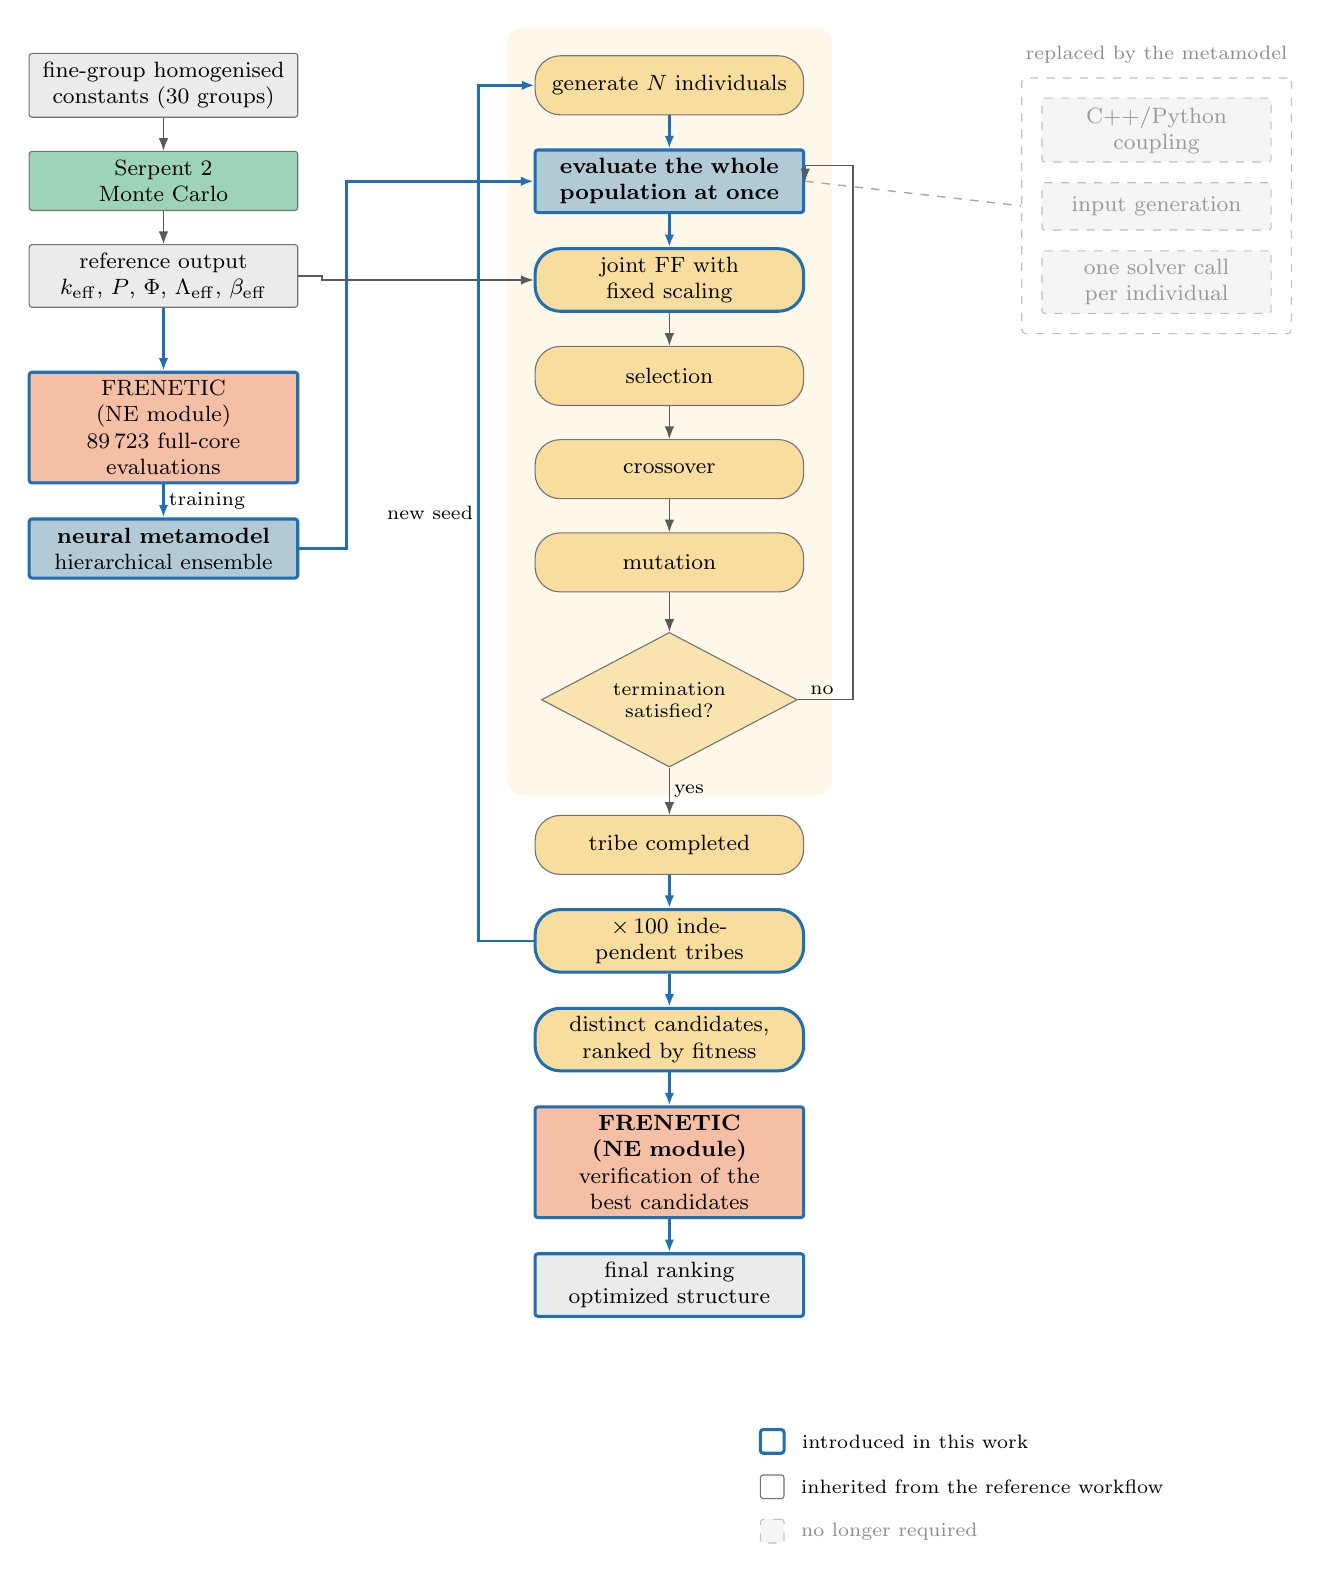
\begin{tikzpicture}[
  font=\footnotesize,
  node distance = 4.2mm and 7mm,
  base/.style    = {rectangle, rounded corners=1pt, align=center, inner sep=3pt,
                    minimum height=7.5mm, text width=32mm},
  old/.style     = {base, draw=black!55, line width=.4pt},
  new/.style     = {base, draw=newc, line width=1.1pt},
  round/.style   = {rounded corners=3.2mm, fill=ga!55},
  serp/.style    = {old, fill=serpent!55},
  frenN/.style   = {new, fill=fren!45},
  netN/.style    = {new, fill=nnc!40},
  greyO/.style   = {old, fill=black!8},
  greyN/.style   = {new, fill=black!8},
  faded/.style   = {base, fill=black!4, draw=black!25, dashed, text=black!40,
                    text width=27mm, minimum height=6mm},
  dec/.style     = {diamond, aspect=1.9, draw=black!55, fill=ga!45, align=center,
                    inner sep=0pt, text width=24mm, font=\scriptsize},
  arO/.style     = {-{Latex[length=1.6mm]}, draw=black!65, line width=.45pt},
  arN/.style     = {-{Latex[length=1.6mm]}, draw=newc, line width=.9pt},
  lbl/.style     = {font=\scriptsize, inner sep=1.5pt},
]

% ── colonna sinistra: riferimento Monte Carlo (invariata) ────────────────
\node[greyO] (fine) {fine-group homogenised\\constants (30 groups)};
\node[serp, below=of fine] (serpent) {Serpent 2\\Monte Carlo};
\node[greyO, below=of serpent] (ref) {reference output\\$k_\mathrm{eff}$, $P$, $\Phi$,
  $\Lambda_\mathrm{eff}$, $\beta_\mathrm{eff}$};

% ── addestramento del metamodello (nuovo) ───────────────────────────────
\node[frenN, below=8mm of ref] (train) {FRENETIC (NE module)\\$89\,723$ full-core\\evaluations};
\node[netN, below=of train] (nn) {\textbf{neural metamodel}\\hierarchical ensemble};

\draw[arO] (fine) -- (serpent);
\draw[arO] (serpent) -- (ref);
\draw[arN] (ref) -- (train);
\draw[arN] (train) -- node[lbl, right] {training} (nn);

% ── ciclo genetico ──────────────────────────────────────────────────────
\node[old, round, right=30mm of fine] (gen) {generate $N$ individuals};
\node[netN, below=of gen] (eval) {\textbf{evaluate the whole\\population at once}};
\node[new, round, fill=ga!55, below=of eval] (ff) {joint FF with\\fixed scaling};
\node[old, round, below=of ff] (sel) {selection};
\node[old, round, below=of sel] (cross) {crossover};
\node[old, round, below=of cross] (mut) {mutation};
\node[dec, below=5mm of mut] (term) {termination\\satisfied?};

\draw[arN] (gen) -- (eval);
\draw[arN] (eval) -- (ff);
\draw[arO] (ff) -- (sel);
\draw[arO] (sel) -- (cross);
\draw[arO] (cross) -- (mut);
\draw[arO] (mut) -- (term);
\draw[arN] (nn.east) -- ++(6mm,0) |- (eval.west);
\draw[arO] (ref.east) -- ++(3mm,0) |- (ff.west);
\draw[arO] (term.east) -- ++(7mm,0) node[lbl, above right, xshift=-6mm] {no}
          |- ([yshift=2mm]eval.east) -- (eval.east);

% ── ciò che il metamodello ha sostituito ────────────────────────────────
\node[faded, right=30mm of eval, yshift=6.5mm] (old1) {C++/Python coupling};
\node[faded, below=2.5mm of old1] (old2) {input generation};
\node[faded, below=2.5mm of old2] (old3) {one solver call\\per individual};
\node[draw=black!25, dashed, rounded corners=1.5pt, inner sep=2.5mm,
      fit=(old1)(old3)] (deadbox) {};
\node[lbl, above=1.2mm of deadbox, text=black!45, align=center, text width=34mm]
     {replaced by the metamodel};
\draw[dashed, draw=black!35, line width=.5pt] (eval.east) -- (deadbox.west);

% ── multi-start e giudizio finale (nuovi) ───────────────────────────────
\node[old, round, below=6mm of term] (tribe) {tribe completed};
\node[new, round, fill=ga!55, below=of tribe] (many) {$\times\,100$ independent tribes};
\node[new, round, fill=ga!55, below=of many] (rank) {distinct candidates,\\ranked by fitness};
\node[frenN, below=of rank] (verify) {\textbf{FRENETIC (NE module)}\\verification of the\\best candidates};
\node[greyN, below=of verify] (out) {final ranking\\optimized structure};

\draw[arO] (term) -- node[lbl, right] {yes} (tribe);
\draw[arN] (tribe) -- (many);
\draw[arN] (many) -- (rank);
\draw[arN] (rank) -- (verify);
\draw[arN] (verify) -- (out);
\draw[arN] (many.west) -- ++(-7mm,0) |- node[lbl, left, pos=.25] {new seed} (gen.west);

% ── legenda ─────────────────────────────────────────────────────────────
\node[new, fill=white, below left=14mm and -32mm of out, text width=3mm,
      minimum height=3mm, inner sep=0pt] (lg1) {};
\node[lbl, right=1.5mm of lg1, anchor=west] {introduced in this work};
\node[old, fill=white, below=2.5mm of lg1, text width=3mm,
      minimum height=3mm, inner sep=0pt] (lg2) {};
\node[lbl, right=1.5mm of lg2, anchor=west] {inherited from the reference workflow};
\node[faded, below=2.5mm of lg2, text width=3mm, minimum height=3mm, inner sep=0pt] (lg3) {};
\node[lbl, right=1.5mm of lg3, anchor=west, text=black!45]
     {no longer required};

\begin{scope}[on background layer]
  \node[fill=ga!12, rounded corners=2mm, fit=(gen)(term)(mut), inner sep=3.5mm] {};
\end{scope}
\end{tikzpicture}
}
  \caption{Workflow adopted in this work, drawn for direct comparison with the
  one of Ref.~\cite{prevMulti}. Boxes and arrows outlined in blue are introduced
  here, those with a thin grey outline are inherited unchanged. Serpent~2
  supplies the fine-group constants and the reference values, and the neutronics
  module of FRENETIC is used once to build the training set of the metamodel.
  Within the genetic loop, the per-individual call to the solver, shown faded on
  the right, is replaced by a single batched evaluation of the whole population
  with the metamodel. The solver returns at the end of the procedure, where it
  recomputes the structures produced by all the independent searches and
  establishes the final ranking.}
  \label{fig:flow}
\end{figure}


\section{Definition of the Optimization Problem}
\label{sec:problem}

\subsection{Reference Data and Fitness Functions}

Serpent~2 is used to generate, for each core configuration, both the reference
values of the integral parameters and the spatially homogenised fine-group
constants, evaluated at isothermal conditions with fuel and coolant at $673$~K.
The data are collapsed onto a fine structure of 30 groups whose boundaries are
extracted from the ECCO-33 grid, chosen so that few groups describe the thermal
and the fast regions where the Monte Carlo statistics are poorest. That
30-group structure constitutes the pool of boundaries available to the
optimization, and the case study is the lead-cooled fast reactor benchmark
coordinated by the Nuclear Energy Agency~\cite{neaBench}.

Three control-rod configurations are considered simultaneously: fully withdrawn,
partially inserted with the absorbing region facing the fuel over a length of
$28$~cm, and fully inserted. For a candidate structure $I$, the agreement with
the Monte Carlo reference is measured by five fitness functions per
configuration~\cite{prevMulti}. Three of them concern integral quantities,
%
\begin{equation}
  f_k^I = \left|k^I - k^\mathrm{MC}\right|\times10^5, \qquad
  f_{\beta}^I = \left|\beta_\mathrm{eff}^I - \beta_\mathrm{eff}^\mathrm{MC}\right|
  \times10^5, \qquad
  f_{\Lambda}^I = \frac{\Lambda_\mathrm{eff}^I -
  \Lambda_\mathrm{eff}^\mathrm{MC}}{\Lambda_\mathrm{eff}^\mathrm{MC}}\times10^2,
  \label{eqn:integral}
\end{equation}
%
namely the multiplication factor, the effective delayed neutron fraction and the
effective neutron generation time, while the remaining two concern the
distributions over the $J$ core assemblies,
%
\begin{equation}
  f_P^I = \sqrt{\sum_{j=1}^{J}\left(\frac{P_j^I-P_j^\mathrm{MC}}
  {P_j^\mathrm{MC}}\right)^{2}}, \qquad
  f_{\Phi}^I = \sqrt{\sum_{g=1}^{G}\sum_{j=1}^{J} w_{g,j}
  \left(\frac{\Phi_{g,j}^I-\Phi_{g,j}^\mathrm{MC}}
  {\Phi_{g,j}^\mathrm{MC}}\right)^{2}},
  \label{eqn:distributed}
\end{equation}
%
the flux being weighted by the total importance $\phi\phi^{\ddagger}/v$. All
five are deviations from the reference, so that smaller values indicate a better
structure.

Since the five quantities differ by orders of magnitude and in range of
variability, each is mapped onto the interval $[1,100]$ by the linear scaling
%
\begin{equation}
  h_L : f \longrightarrow 1 + 99\,
  \frac{f-\min_{\forall I\in E}\left(f^I\right)}
       {\max_{\forall I\in E}\left(f^I\right)-\min_{\forall I\in E}\left(f^I\right)},
  \label{eqn:scaling}
\end{equation}
%
where $E$ denotes the set of solutions evaluated so far, and the joint fitness
of a candidate is the product of the fifteen scaled terms, five for each of the
three configurations,
%
\begin{equation}
  FF^I = \prod_{c\in\{\mathrm{out},\,\mathrm{partial},\,\mathrm{in}\}}
  h_L\!\left(f_{k,c}^I\right) h_L\!\left(f_{P,c}^I\right)
  h_L\!\left(f_{\Phi,c}^I\right) h_L\!\left(f_{\Lambda,c}^I\right)
  h_L\!\left(f_{\beta,c}^I\right).
  \label{eqn:joint}
\end{equation}
%
Before the scaling, the three integral fitness functions are clipped from below
at a value of ten, which is of the order of the Monte Carlo uncertainty on the
corresponding quantity, and the flux fitness function is replaced by its
base-ten logarithm floored at unity. Both operations prevent a single term
already at the level of the reference uncertainty from dominating the product,
and are applied identically to the reference values and to the candidate ones.

\subsection{Chromosome Representation}

The optimization variable is the set of internal boundaries retained from the
fine structure. Of the 31 boundaries of the 30-group mesh the two extremes are
fixed, so that a candidate structure corresponds to a subset of the remaining
$H-1=29$ internal boundaries and the design space contains
$2^{29}\approx5.4\times10^{8}$ elements.

The representation adopted here is the polyploid encoding of
Ref.~\cite{prevMulti}, reproduced in full because it determines both the
behaviour of the genetic operators and the input of the metamodel. A chromosome
consists of two sets. The first, $\gamma_0$, is a single gene holding the number
of groups $G$ of the structure, constrained to $4\le G\le20$. The second,
$\gamma_1$, is polyploid and contains $P=4$ arrays of $H-1=29$ genes each, one
gene per internal boundary, whose alleles take integer values in $\{0,1,2\}$. An
individual is therefore described by $1+P(H-1)=117$ variables.

Decoding proceeds in two steps. For each internal boundary $i$ the $P$ arrays
are summed into a score
%
\begin{equation}
  s_i = \sum_{p=1}^{P} \gamma_{1,p,i}, \qquad i = 1,\dots,H-1,
  \label{eqn:score}
\end{equation}
%
and the $G-1$ boundaries with the highest score are retained, ties being
resolved by increasing energy index. The polyploid structure gives each boundary
a graded rather than binary expression, so that a boundary can be strengthened
or weakened by mutation without being switched on or off abruptly, which
smooths the effect of the genetic operators on the decoded structure. A repair
operator enforces the bounds on $G$ and the validity of the alleles after
crossover and mutation.


\section{The Metamodel}
\label{sec:metamodel}

\subsection{Training Set}

The metamodel is trained on 91\,723 distinct structures for which the
neutronics module of FRENETIC has been run over the three configurations. The
set was assembled starting from a space-filling pool and enlarged in successive
batches, the configurations to be simulated next being chosen by the
disagreement among the members of an ensemble of five networks, averaged over
the nine quantities that the model predicts least accurately, namely the
multiplication factor, the flux and the generation time for the three
configurations. A further 1\,700 structures form an external validation set
which is never used in training, nor for early stopping, nor for any
hyperparameter decision. Every accuracy figure quoted in this work refers to
that set.

\subsection{Architecture}

The fifteen fitness functions are not independent, since they group into five
physical families, each evaluated for the same three core states. The network
reproduces that organisation. A shared trunk of three fully connected layers of
$1024$, $512$ and $256$ neurons receives the 29-bit description of the structure
together with the number of groups. The trunk feeds five family-level branches
of $128$ and $64$ neurons, each of which feeds three configuration-level
branches of $32$ neurons terminating in the corresponding output. Parameters are
thus shared to the extent that the physics shares them and specialised where it
does not. An ablation performed on the same data gives a mean coefficient of
determination of $0.9852$ for a single-headed network, $0.9882$ when only the
five families are separated, and $0.9894$ for the full hierarchy.

Twelve of the fifteen outputs span several orders of magnitude and are learned
as $\log_{10}(y+10^{-6})$, while the three power fitness functions are learned
directly. Predictions are averaged over an ensemble of five networks trained
from different random initialisations~\cite{deepEnsembles}. The disagreement
among the members of the ensemble also provides the criterion used to select the
configurations added to the training set.

\subsection{Training and Accuracy}

The networks are trained in PyTorch~\cite{pytorch} with the AdamW
optimizer~\cite{adamw} and no weight decay, in four stages of decreasing
learning rate, $3\times10^{-3}$, $3\times10^{-4}$, $10^{-4}$ and
$3\times10^{-5}$, each stopped on the validation loss. The staged schedule
proves considerably more effective than a constant learning rate: the same
architecture trained at $3\times10^{-3}$ with early stopping reaches a median
relative error of $0.715\%$, against $0.422\%$ with the staged decay on the same
data, a reduction of $41\%$ which exceeds the combined effect of all the
architectural refinements described above. A control run performed with the
staged schedule and no additional data reproduces the improvement exactly, which
confirms that it originates in the schedule and not in the training set.

Table~\ref{tab:accuracy} reports the accuracy of the final ensemble for each
output and Fig.~\ref{fig:scatter} the corresponding predicted against reference
values. The mean coefficient of determination is $0.99634$ and the median
relative error $0.403\%$. The accuracy is not uniform across the fifteen
quantities: the power fitness functions are reproduced to better than $0.2\%$
and the delayed neutron fraction to about $0.4\%$, while the flux functions,
which are the least accurate, lie between $2.0$ and $2.3\%$.

\begin{figure}[htbp]
  \centering
  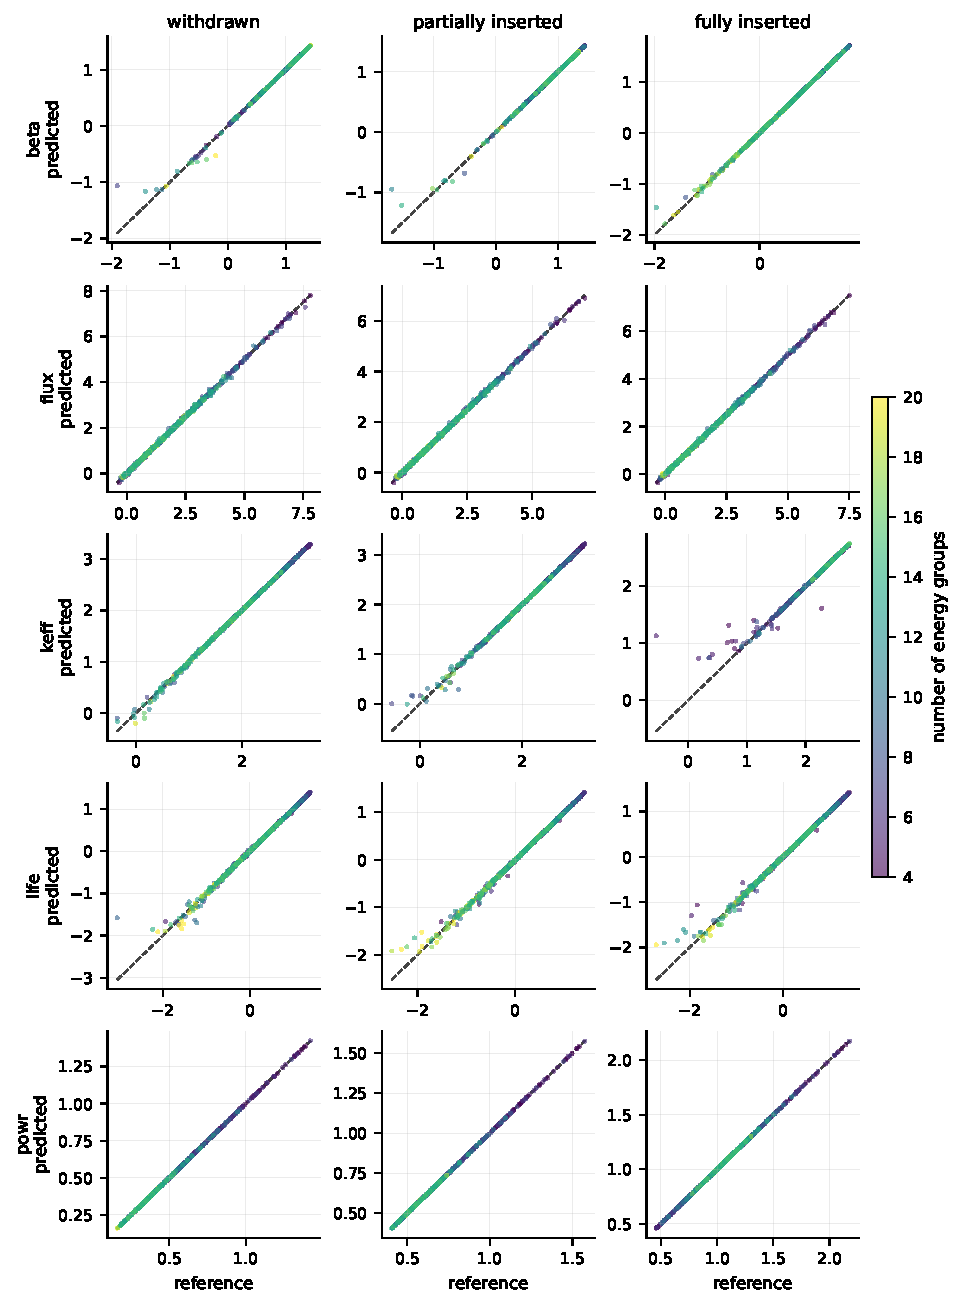
\includegraphics[width=132mm]{figs/fig_scatter.pdf}
  \caption{Predicted against reference values of the fifteen fitness functions
  for the 1700 configurations of the external validation set. Rows correspond to
  the five physical families and columns to the three control-rod
  configurations. Colour encodes the number of energy groups of the structure.
  Axes are in the space in which the network is trained, logarithmic for every
  quantity except the power. The dashed line is the identity.}
  \label{fig:scatter}
\end{figure}

The size of the training set was established by a retrospective experiment
rather than assumed. Starting from a random subset of $10\,000$ configurations,
the campaign was replayed by repeatedly training an ensemble, ranking the
remaining configurations by ensemble disagreement and adding the ten thousand
most uncertain ones. The resulting curve, Fig.~\ref{fig:learning}, decreases
steadily and does not flatten before the pool is exhausted, which indicates
that the accuracy is still limited by the amount of available data rather than
by the model. The campaign was stopped because the pool was exhausted, and the
error obtained with the full set is sufficient for the use made of the metamodel
in the following, as discussed in Sec.~\ref{sec:workflow}.

\begin{figure}[htbp]
  \centering
  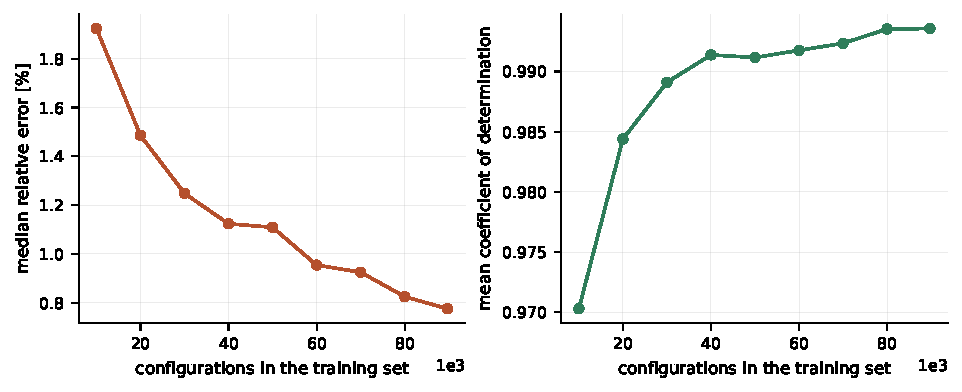
\includegraphics[width=135mm]{figs/fig_learning.pdf}
  \caption{External validation error as a function of the size of the training
  set, obtained by replaying the acquisition campaign on the assembled data.
  Left, median relative error; right, mean coefficient of determination over the
  fifteen outputs. A reduced training protocol was adopted so that the points
  are comparable with one another, and the absolute level is consequently higher
  than that of the final five-network ensemble.}
  \label{fig:learning}
\end{figure}

\subsection{The Regime of Reduced Accuracy}
\label{sec:limit}

The residual error is not distributed uniformly over the design space. It
concentrates at small values of the reactivity and kinetics fitness functions
and, for the flux, at large values. Since small fitness values identify the best
structures, the behaviour deserves a quantitative explanation.

Three candidate causes were examined and each was excluded by direct
measurement, as summarised in Table~\ref{tab:hypotheses}. The labels carry no
statistical noise, since of the configurations present in more than one data
file, 21\,440 in total, the spread is $0.0000\%$ on every output, and an
independent re-run of the solver reproduces stored values to all digits. The
regime is not under-sampled: dividing the range of the reference value into
bands and comparing the two extreme ones, which the validation set samples with
the same number of points, the band where the error is largest contains
$13\,205$ training configurations while the band at the opposite end, where the
error is one third as large, contains $5\,317$. The input representation is not
deficient either, since augmenting the description with 65 physics-informed
descriptors, namely the lethargy widths of the condensed groups, the variation
of the reference flux shape within each of them weighted by the importance, and
the widths of the groups containing the sharpest spectral features, makes the
model worse rather than better, $0.473\%$ against $0.403\%$ on the same data
and with the same training recipe. A network of this capacity evidently
constructs such features internally where they are useful.

The explanation lies in the target function itself. Searching the data set for
pairs of structures differing by exactly one boundary yields 55\,058 such pairs.
The median change of the base-ten logarithm of the fitness function across a
pair amounts to $0.414$ decades in the lowest band of multiplication-factor
deviations, against $0.024$ decades in the highest, a factor of seventeen, and
to $0.395$ against $0.044$ decades for the generation time.
Figure~\ref{fig:smallvalue} shows that the error of the metamodel follows this
local steepness across all five families, including the flux, which is steepest
at large values and is indeed least accurate there.

The physical interpretation is direct. A small fitness value means that the
condensed calculation reproduces the reference almost exactly, an agreement
achieved through a fine cancellation of the errors committed in the individual
groups. Such cancellations are fragile, and displacing a single boundary
destroys them. A smooth interpolator cannot follow a function that varies by
half a decade under a one-bit change of its input, and no amount of additional
data of the same kind will remove the limitation. This is the reason why the
workflow described in the next section does not rely on the metamodel for its
conclusions.

\begin{figure}[htbp]
  \centering
  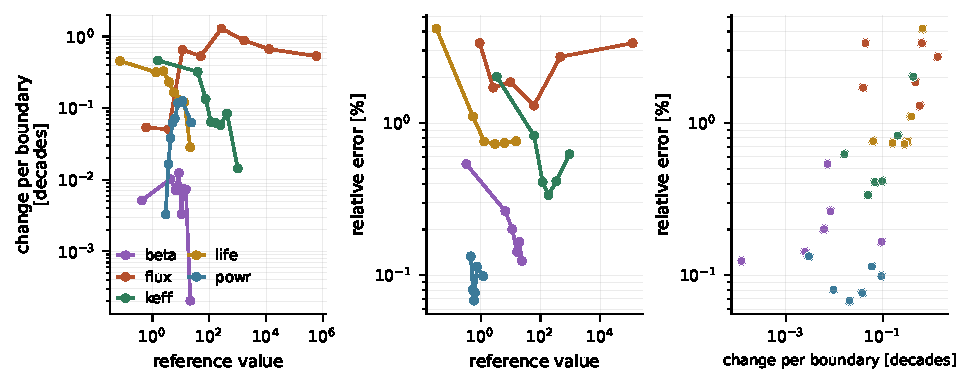
\includegraphics[width=150mm]{figs/fig_steepness.pdf}
  \caption{Left, steepness of the target measured on the pairs of structures
  that differ by exactly one boundary, as the median change of the base-ten
  logarithm of the fitness function across a pair. Centre, median relative error
  of the metamodel over the same bands of the reference value. Right, the two
  quantities plotted against each other, one point per band and family. The
  error of the metamodel follows the local steepness of the target rather than
  the magnitude of the quantity, which is why the flux behaves in the opposite
  way with respect to the other four families.}
  \label{fig:smallvalue}
\end{figure}


\section{Workflow}
\label{sec:workflow}

\subsection{A Fitness on a Fixed Scale}
\label{sec:canonical}

The scaling of Eq.~(\ref{eqn:scaling}) employs the extreme values encountered so
far in the run. The choice keeps the comparison internally consistent within a
generation, but it makes the scale itself dependent on how much a given run has
explored, so that the joint fitness values of two runs are not directly
comparable. The effect is measurable: a search of 500 generations reports a
final fitness worse than one of 300 generations on the same problem, for no
other reason than having widened its own scaling window.

Since the analysis presented here rests on the comparison of a hundred
independent searches, the two extremes of Eq.~(\ref{eqn:scaling}) are computed
once from all the available configurations and then held fixed. The resulting
canonical fitness is comparable across runs and stationary within a run. Its
effect on the behaviour of the algorithm was verified by repeating thirty
searches with each formulation from identical seeds and comparing the outcomes
on the same scale. The best structure found is identical in the two cases,
$8.3175\times10^{6}$, while the median outcome improves by $4.8\%$ and the
number of distinct structures rises from $23$ to $26$ out of thirty. The fixed
scale therefore does not alter where the algorithm converges, and improves
marginally the quality of the typical run. It also removes the need to
re-evaluate the whole population at every generation, which was introduced in
the original formulation to compensate for the moving scale, with a reduction of
the computing time by a factor of $1.5$.

\subsection{Multiple Independent Searches}

The searches use a population of 100 individuals over 100 generations, with
tournament selection, two-point crossover, integer random mutation at $0.05$ per
gene and the repair operator described in Sec.~\ref{sec:problem}. The
implementation is built on the pymoo library~\cite{pymoo} and reproduces the
scheme of Ref.~\cite{prevMulti} in its representation, operators and fitness
functions. The population and generation counts were established by
measurement: a population of 40 individuals yields a median final fitness $1.6$
times worse, a population of 200 improves it by $3\%$, and the median search
reaches within $1\%$ of its own final value by generation 32, while seven
searches out of a hundred are still improving after generation 90.

One implementation detail deserves mention because it affects reproducibility.
The sampling and mutation operators of this problem draw from the global random
generator, which the optimization library does not seed, so that the seed passed
to the optimizer has no effect and successive runs are not reproducible.
Seeding the global generator explicitly before each tribe restores bit-level
reproducibility, and all results presented here can be regenerated exactly.

The searches are mutually independent and are executed in parallel. One hundred
of them require $77$~s on eight processes, so that the cost of exploring the
design space a hundred times over is smaller than the cost of two evaluations of
the reference solver.

\subsection{Verification with the Reference Solver}

The distinct structures produced by the searches are ranked by canonical fitness
and submitted to FRENETIC, and the ranking reported in the following is the one
obtained from the recomputed values. No quantity discussed in
Sec.~\ref{sec:results} is a prediction of the metamodel. This arrangement is
deliberate and follows from Sec.~\ref{sec:limit}: the metamodel is accurate
enough to order the candidates and thus to identify a short list worth a
full-core calculation, which is a considerably weaker requirement than
predicting the fitness of the best structures to the precision needed to rank
them among themselves.


\section{Results and Discussion}
\label{sec:results}

\subsection{Behaviour of the Searches}

The hundred searches produced 67 distinct structures, with a number of groups
between 12 and 20. Figure~\ref{fig:search} shows their convergence on the common
canonical scale, the distribution of the generation at which each search reaches
within $1\%$ of its own final value, and the position of the outcomes in the
plane of group count against fitness. A quarter of the searches finish within
$5\%$ of the best predicted fitness and the median one is $15\%$ worse, which
confirms the observation of Ref.~\cite{prevMulti} on a much larger sample: a
single search returns a good structure with substantial probability, but which
structure it returns is not determined by the problem alone.

\begin{figure}[htbp]
  \centering
  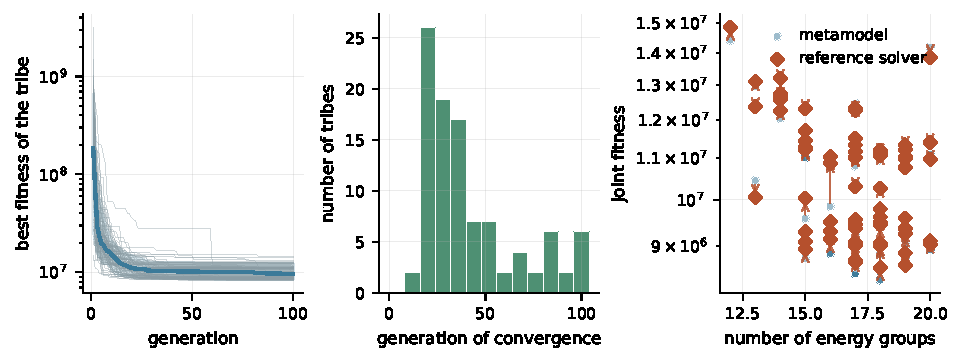
\includegraphics[width=150mm]{figs/fig_search.pdf}
  \caption{Behaviour of the hundred independent searches. Left, best joint
  fitness against generation, one line per search, with the median and the band
  between the tenth and ninetieth percentiles. Centre, distribution of the
  generation at which a search first comes within one per cent of its own final
  value. Right, position of the outcomes in the plane of group count against
  joint fitness, the arrows joining the value predicted by the metamodel to the
  one obtained from the reference solver for the verified candidates.}
  \label{fig:search}
\end{figure}

The internal dynamics of a single search are illustrated in
Fig.~\ref{fig:tribe}. The initial population is heterogeneous, most boundaries
being present in about half of the individuals, and within a dozen generations
the population crystallises, each boundary being either adopted by nearly every
individual or abandoned by nearly all of them. Two later events, visible around
generations 22 and 76, show a boundary that had been fixed being re-opened and
replaced, which indicates that crossover and mutation continue to restructure
the solution after the joint fitness has apparently settled.

\begin{figure}[htbp]
  \centering
  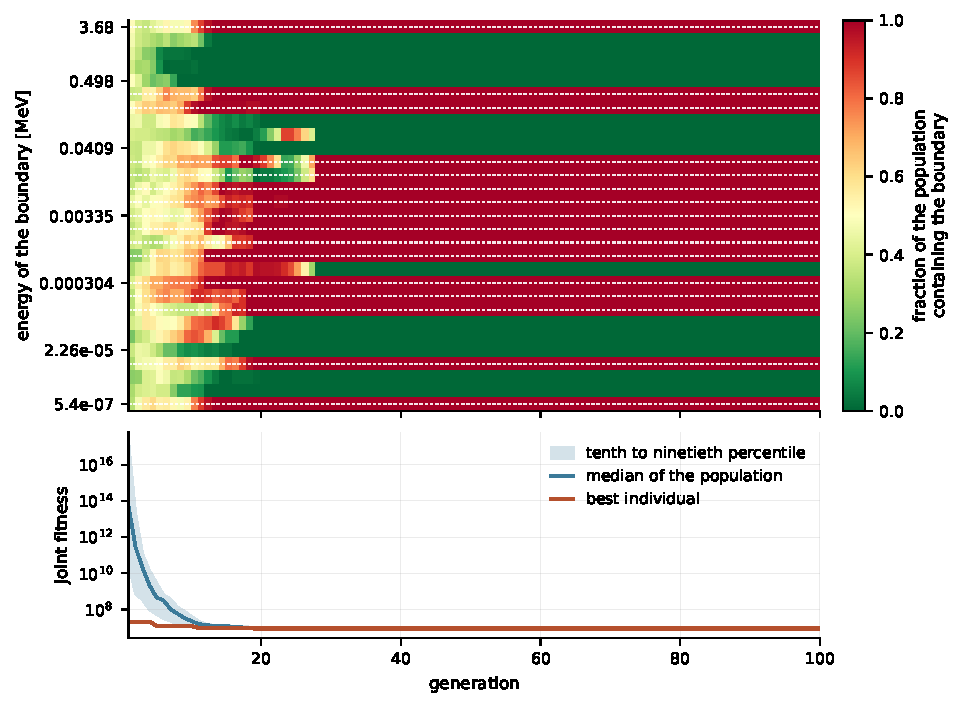
\includegraphics[width=150mm]{figs/fig_tribe.pdf}
  \caption{Evolution of a single search. Above, fraction of the population
  containing each internal boundary, generation by generation, from green when
  the boundary is absent from the whole population to red when every individual
  carries it, the white dotted lines marking the boundaries of the final
  structure of this search. Below, on the same generation axis, joint fitness of
  the population as the band between the tenth and ninetieth percentiles, its
  median and the best individual.}
  \label{fig:tribe}
\end{figure}

\subsection{Two Families of Solutions}

The 67 distinct structures do not form a single group. Clustering them by
Hamming distance separates two families whose mean internal distance is $5.0$
boundaries against $10.4$ between them, and the searches divide almost equally
between the two, 53 against 47. The separation is not a matter of group count,
since the two families span overlapping ranges of $G$, but of a coherent block
of mutually exclusive choices in the fast region of the spectrum, as reported in
Table~\ref{tab:families} and visible in the right panel of
Fig.~\ref{fig:structure}. The boundaries at $2.231$ and $0.302$~MeV never occur
together in any of the 67 structures, with a correlation coefficient of $-1.00$,
while the boundary at $3.679$~MeV occurs together with the one at $0.302$~MeV
and with the thermal boundary at $5.4\times10^{-7}$~MeV, with correlations of
$+0.97$ and $+0.94$. One family therefore adopts the block formed by $3.679$ and
$0.302$~MeV together with the thermal cut, the other adopts $2.231$~MeV together
with a boundary at $1.371\times10^{-5}$~MeV.

The two blocks are alternative and self-consistent. The boundaries at $3.679$
and $2.231$~MeV are adjacent in the fine mesh, so that retaining both would
subdivide a region which carries little flux, and once one of the two is adopted
the placement of the remaining boundaries adapts to it. No single mutation
converts a structure of one family into a structure of the other, which explains
why a search remains within the family in which its initial population happens
to fall.

The two families are not equivalent. Verifying with FRENETIC the six best
members of the less favourable one gives a median true fitness of
$1.055\times10^{7}$ against $9.105\times10^{6}$ for the other, a difference of
$16\%$. The origin of the difference can be traced to the way the two families
condense the spectrum. For each structure the variation of the reference flux
shape within its groups was computed and weighted by the total importance
$\phi\phi^{\ddagger}/v$ of the group, which is the weight with which the flux
fitness function of Eq.~(\ref{eqn:distributed}) counts an error. The result,
reported in Table~\ref{tab:families}, is $0.138$ for the better family against
$0.377$ for the other. Where it matters to the objective, the structures of the
better family follow the shape of the spectrum more closely, and the difference
in fitness follows. The same quantity weighted by the bare flux separates the
two families much less, $0.212$ against $0.247$, which indicates that it is the
importance weighting, and not the flux alone, that decides which of the two
blocks is preferable.

\begin{figure}[htbp]
  \centering
  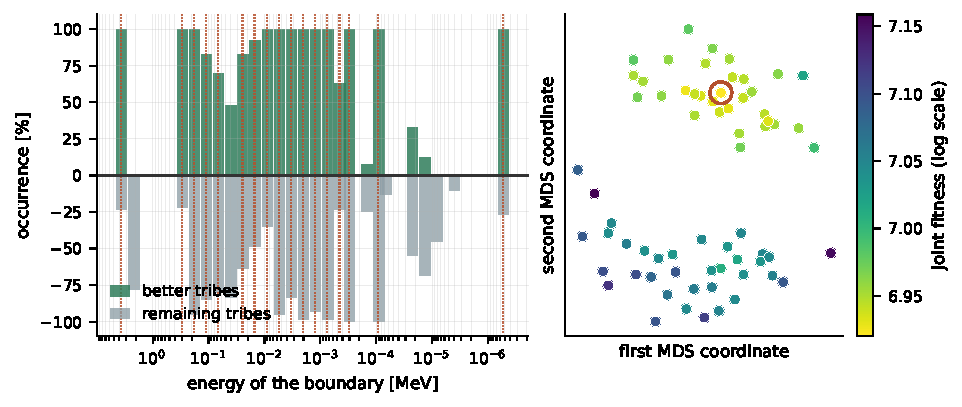
\includegraphics[width=150mm]{figs/fig_structure.pdf}
  \caption{Left, frequency with which each internal boundary of the fine mesh
  appears among the better searches, taken as the best forty per cent and
  plotted upward, and among the remaining ones, plotted downward, the dotted
  vertical lines marking the boundaries of the best structure found. Right,
  two-dimensional multidimensional scaling of the Hamming distance between the
  distinct structures, coloured by joint fitness, the circled point being the
  best structure. The two separated groups are the two families discussed in the
  text.}
  \label{fig:structure}
\end{figure}

\subsection{Recurring Features of the Optimized Structures}
\label{sec:patterns}

Beyond the separation into families, the 67 structures display regularities
which can be examined collectively, and which constitute the general information
that a single search cannot provide.

Seven boundaries occur in more than $90\%$ of the structures and form a
consensus skeleton, located at $0.1832$, $5.53\times10^{-3}$,
$2.04\times10^{-3}$, $1.23\times10^{-3}$, $7.49\times10^{-4}$,
$3.04\times10^{-4}$ and $9.17\times10^{-5}$~MeV, that is entirely within the
epithermal region. Five boundaries are never selected, three of them in the fast
region at $1.353$, $0.8208$ and $0.4979$~MeV and two at $4.02\times10^{-5}$ and
$4\times10^{-6}$~MeV. The remaining seventeen are used with intermediate
frequency and account for the variability among the solutions.

The placement of the recurring boundaries admits a physical reading which is not
the one that intuition suggests. A natural expectation is that boundaries should
be placed where the spectrum changes shape most abruptly, since a single group
cannot represent a rapidly varying flux, and that they should follow the flux
itself, since a group carrying little flux contributes little to the reaction
rates. Neither expectation is confirmed. The rank correlation between the
frequency with which a boundary is selected and the variation of the flux shape
across it is negative, $-0.51$ with a probability of $5\times10^{-3}$ under the
null hypothesis, and the correlation with the flux surrounding the boundary is
not significant, $+0.17$ with a probability of $0.37$. The three boundaries
associated with the sharpest variations of shape in the fast region, at $1.353$,
$0.8208$ and $0.4979$~MeV, are never used, although together they lie where
$18\%$ of the flux is found.

The quantity that does predict the placement is the one that the objective
function itself uses as a weight. The flux fitness function of
Eq.~(\ref{eqn:distributed}) measures the flux error of every group weighted by
the total importance $\phi\phi^{\ddagger}/v$, so that the relevant measure of
how much a group matters is not how much flux it carries but how much importance
it carries. The rank correlation between the selection frequency of a boundary
and the importance surrounding it is $+0.53$, with a probability of
$3\times10^{-3}$. The three boundaries of the fast region that are never
selected lie where the importance is $0.68$, $1.57$ and $2.32\%$, against values
between $1.86$ and $5.03\%$ for the boundaries of the consensus skeleton. The
distinction between the two readings is sharp in that region. The adjoint flux
of this core varies by less than a factor of two over the whole energy range, so
that the importance follows essentially the ratio $\phi/v$: the fast groups
carry a substantial part of the flux but, at those speeds, only a small part of
the importance, the ratio between the two fractions rising monotonically from
$0.10$ in the highest group to unity around $10$~keV. The optimizer places its
boundaries according to the second quantity and not the first.

The tendency can be stated more directly. Computing for each structure the
coefficient of variation of the importance contained in its groups gives $0.553$
for the ten best structures against $0.835$ for random structures with the same
number of groups, so that the optimized structures are $1.5$ times more even.
The same measure applied to the bare flux gives $1.104$ against $1.217$, a
difference of only $10\%$. The optimization therefore moves towards an
equipartition of the importance among the groups, a criterion which was never
imposed explicitly and which follows from the weighting of
Eq.~(\ref{eqn:distributed}).

\begin{figure}[htbp]
  \centering
  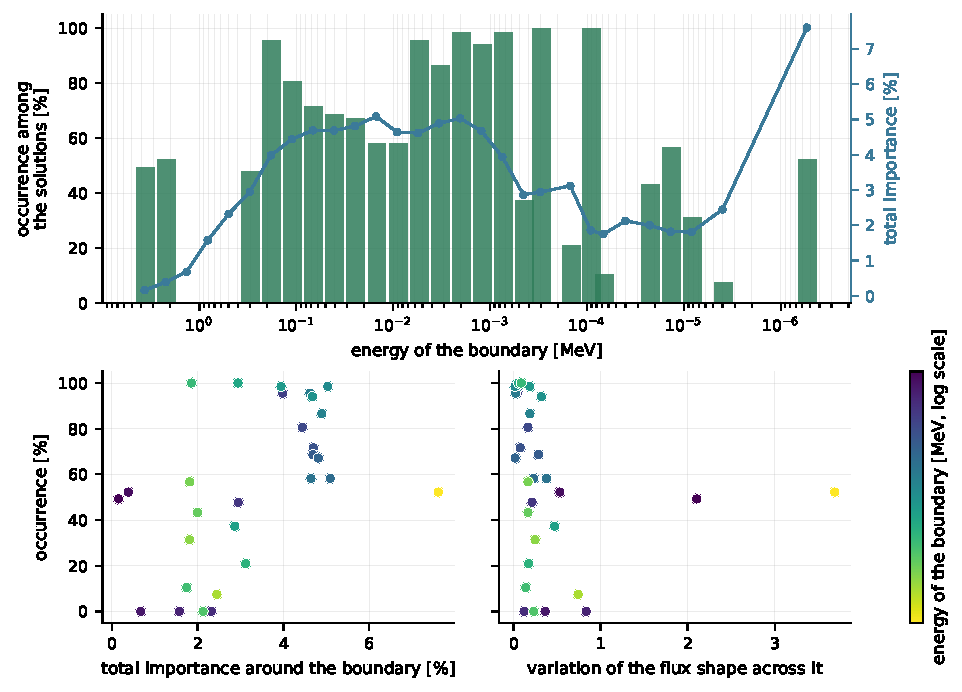
\includegraphics[width=150mm]{figs/fig_boundaries.pdf}
  \caption{Recurring features of the optimized structures. Above, frequency with
  which each internal boundary is selected among the 67 distinct structures, in
  green, and total importance surrounding each boundary on the same energy axis,
  in blue. Below, the same frequency plotted against the surrounding importance
  and against the variation of the flux shape across the boundary, the colour
  encoding the energy of the boundary. The frequency increases with the
  importance and, if anything, decreases with the sharpness of the spectral
  variation.}
  \label{fig:boundaries}
\end{figure}

\subsection{Number of Groups}

Repeating the searches with the number of groups constrained gives the fitness
attainable as a function of $G$, shown in Fig.~\ref{fig:tradeoff} with every
point verified by FRENETIC. The attainable fitness improves by a factor of $4.3$
between $G=8$ and $G=14$ and is essentially flat thereafter, the whole range
from $G=14$ to $G=20$ lying within $7\%$. Fourteen groups are therefore
sufficient for this core and this set of fitness functions, and the additional
groups used by the best structures bring little further benefit. Thirteen
constrained optimizations of this kind require four minutes on the metamodel and
would require of the order of five thousand core-hours on the solver.

\begin{figure}[htbp]
  \centering
  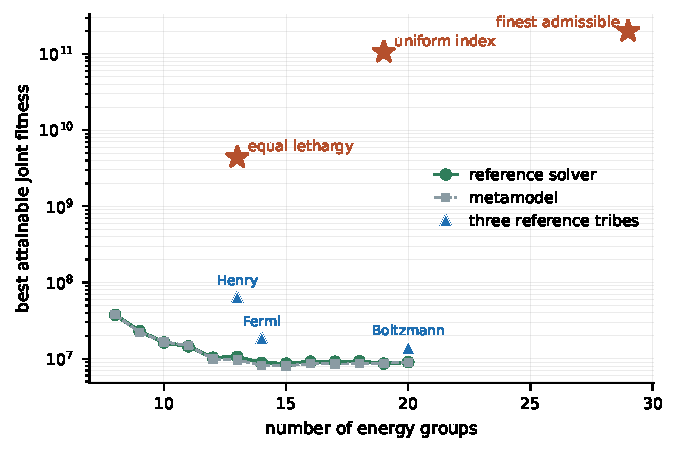
\includegraphics[width=110mm]{figs/fig_tradeoff.pdf}
  \caption{Best attainable joint fitness as a function of the number of energy
  groups, obtained by repeating the searches with the group count constrained.
  Each point of the solid curve was verified with the reference solver, while
  the dashed curve is the corresponding prediction of the metamodel. The stars
  mark the two standard constructions discussed in the text.}
  \label{fig:tradeoff}
\end{figure}

\subsection{Comparison with Reference Structures}

The best verified structure uses $G=18$ groups and reaches a canonical fitness
of $8.5582\times10^{6}$, with internal boundaries at $3.679$, $0.302$, $0.1832$,
$0.1111$, $6.738\times10^{-2}$, $2.479\times10^{-2}$, $1.503\times10^{-2}$,
$9.119\times10^{-3}$, $5.531\times10^{-3}$, $3.355\times10^{-3}$,
$2.035\times10^{-3}$, $1.234\times10^{-3}$, $7.485\times10^{-4}$,
$4.540\times10^{-4}$, $3.043\times10^{-4}$, $9.166\times10^{-5}$ and
$5.4\times10^{-7}$~MeV. It belongs to the better of the two families and
contains the whole consensus skeleton. It outperforms every one of the
$124\,693$ configurations computed to date, by $15.8\%$ with respect to the best
among them, and none of those configurations reaches its fitness.

Table~\ref{tab:standard} compares it with three reference constructions. A
structure with uniformly spaced boundary indices and the same number of
boundaries is worse by a factor of $1.2\times10^{4}$, and one with uniform
lethargy spacing by a factor of $5.1\times10^{2}$. It is worth noting that a
uniform-lethargy structure cannot be built with 19 boundaries on this fine mesh,
since the 30 fine groups are not themselves equally spaced in lethargy, so that
equally spaced targets collapse onto repeated boundaries and only 13 survive.
The fine mesh constrains which regular structures can be constructed at all.

The third reference is the finest structure the framework admits. The collapsing
routine requires the condensed structure to contain fewer groups than the fine
one, so that $G=30$ is not a legitimate option and the limit is $G=29$, obtained
by suppressing a single boundary. All twenty-nine such structures were
evaluated. The best of them, obtained by suppressing the boundary at
$0.4979$~MeV, reaches a canonical fitness of $1.99\times10^{11}$, the median is
$6.56\times10^{11}$ and the worst, obtained by suppressing the thermal boundary
at $5.4\times10^{-7}$~MeV, is $2.61\times10^{14}$.

The optimized 18-group structure is therefore better than the best 29-group
structure by more than four orders of magnitude. The result is not paradoxical.
The neutronics module of FRENETIC solves the multi-group diffusion equation, and
a structure that retains almost all the fine boundaries produces groups that are
optically thin, a regime in which diffusion theory is known to perform poorly.
The observation confirms and quantifies the remark of Ref.~\cite{prevMulti} that
the algorithm drives the solutions towards a relatively high number of groups
with a counter-intuitive outcome. It also provides the strongest justification
for the optimization itself, since the finest available structure is not merely
suboptimal but substantially worse than a carefully chosen coarse one.

\subsection{Accuracy of the Metamodel on the Proposed Structures}

Table~\ref{tab:ranking} reports the fifteen distinct candidates that were
recomputed with FRENETIC. The median difference between the predicted and the
true joint fitness is $3.0\%$, and the structure that the metamodel ranks first
is also the best according to the solver. The agreement should not be
over-interpreted, since the second-ranked structure lies only $0.55\%$ behind
the first in true fitness, a margin well below the resolution of the metamodel.
What the comparison establishes is that the ordering produced by the metamodel
is reliable enough to identify a short list containing the best structures,
which is what the workflow requires of it.

The distribution of the error over the fifteen quantities, in the right panel of
Fig.~\ref{fig:bias}, shows that ten of them are predicted to better than
$1.3\%$ on the proposed structures, while the multiplication factor with the
rods partially inserted and the flux with the rods fully inserted reach median
errors of $8.0\%$ and $6.9\%$. The first of these is the regime of
reduced accuracy characterised in Sec.~\ref{sec:limit}, appearing here in
operation rather than in diagnosis, and its magnitude on the proposed structures
is consistent with what the analysis of the target steepness predicts.

The left panel shows a systematic feature of surrogate-driven optimization which
is worth recording. Thirteen of the fifteen predictions underestimate the true
fitness. A search that minimises a predicted quantity is attracted both to
genuinely good structures and to structures whose quality the metamodel
overestimates, and cannot distinguish between the two. The bias is modest in
magnitude, the median difference being $3.0\%$, and it does not affect the
conclusions because every reported quantity comes from the solver, but it
explains why the verification stage becomes more rather than less necessary as
the number of searches grows.

\begin{figure}[htbp]
  \centering
  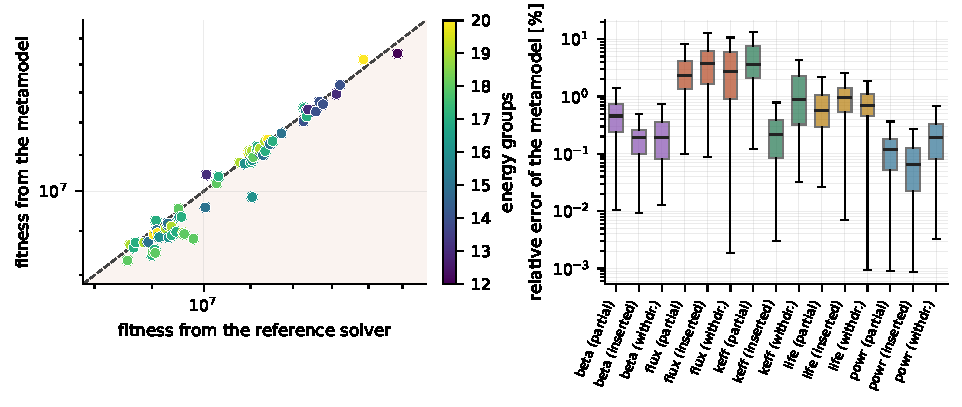
\includegraphics[width=150mm]{figs/fig_bias.pdf}
  \caption{Left, joint fitness predicted by the metamodel against the value
  obtained from the reference solver for the verified candidates, the shaded
  region indicating underestimation and the colour the number of energy groups.
  Right, distribution of the relative error of the metamodel on the same
  candidates, quantity by quantity, with boxes spanning the interquartile range
  and whiskers the extremes.}
  \label{fig:bias}
\end{figure}

\subsection{Computational Cost}

Table~\ref{tab:cost} summarises the computational budget. Assembling the
training set required approximately $3\,516$ core-hours of FRENETIC, while a
single search evaluated directly on the solver would require $383$. The
metamodel therefore becomes advantageous beyond approximately nine searches, and
the analysis presented here, which comprises one hundred searches together with
thirteen constrained optimizations, would have required of the order of
$43\,000$ core-hours without it. The verification of the candidates, which is
the only part of the procedure that still calls the solver during the analysis,
accounts for a few core-hours.

The comparison is favourable also in the terms in which the problem was posed.
The training set is an asset that outlives the single optimization: once
assembled, it supports the constrained analyses of Sec.~\ref{sec:results}, any
subsequent re-optimization with modified fitness functions, and the
characterization of the landscape presented in Sec.~\ref{sec:patterns}, none of
which would be affordable otherwise.


\section{Conclusions}
\label{sec:conclusion}

The dependence of the optimized energy structure on the random seed, reported in
the multi-configuration study which precedes this work, has been investigated by
performing one hundred independent searches instead of three. The number was
made accessible by a neural metamodel of the fifteen fitness functions, trained
on 91\,723 full-core evaluations and accurate to a median relative error of
$0.403\%$ on configurations never seen during training, while every structure
produced by the searches was recomputed with the reference solver, so that the
conclusions rest on FRENETIC and not on the metamodel.

The landscape turns out to be organised rather than merely rugged. The searches
converge to 67 distinct structures which separate into two families, defined by
a block of mutually exclusive boundary choices in the fast region, between which
no single mutation can pass and which differ by $16\%$ in true fitness. Within
that organisation the structures share a skeleton of seven boundaries present in
more than nine cases out of ten, all located in the epithermal region, while
five boundaries are never selected. The placement of the recurring boundaries
follows the neutron importance with which the objective function weights the
flux error, and not the sharpness of the spectral variation nor the flux itself,
and the optimized structures distribute that importance among their groups one
and a half times more evenly than random structures with the same number of
groups.

The best structure identified employs eighteen groups. It improves on the best
of the $124\,693$ configurations computed so far by $15.8\%$, on structures
built by uniform spacing rules by two to four orders of magnitude, and on the
finest structure the collapsing procedure admits, with twenty-nine groups, by
more than four orders of magnitude. The last comparison shows that retaining
almost all the fine boundaries is not a conservative choice, since it produces
optically thin groups for which the diffusion solver is inaccurate, and provides
the clearest justification for optimizing the structure rather than refining it.
The attainable fitness was also found to saturate beyond fourteen groups, so
that the number of groups can be chosen on the grounds of computational cost
once that threshold is exceeded.


\section*{Acknowledgements}
% TODO: ringraziamenti e finanziamenti


\begin{table}[htbp]
\centering
\caption{Metamodel accuracy on the external validation set, 1700 configurations
never used in training nor for early stopping. The coefficient of determination
is computed in the space in which the network is trained; the relative error is
in physical units.}
\label{tab:accuracy}
\begin{tabular}{|lcc|lcc|}
\hline
Output & $R^2$ & Rel.\ err.\ [\%] & Output & $R^2$ & Rel.\ err.\ [\%] \\ \hline
    beta\_CRin0 & 0.99762 & 0.195 & beta\_CRin55 & 0.99938 & 0.399 \\
    beta\_CRout & 0.99585 & 0.165 & flux\_CRin0 & 0.99943 & 2.114 \\
    flux\_CRin55 & 0.99945 & 2.431 & flux\_CRout & 0.99940 & 2.413 \\
    keff\_CRin0 & 0.99524 & 0.559 & keff\_CRin55 & 0.97926 & 0.222 \\
    keff\_CRout & 0.99918 & 0.750 & life\_CRin0 & 0.99717 & 0.875 \\
    life\_CRin55 & 0.99134 & 0.884 & life\_CRout & 0.99155 & 0.948 \\
    powr\_CRin0 & 0.99994 & 0.099 & powr\_CRin55 & 0.99995 & 0.070 \\
    powr\_CRout & 0.99994 & 0.192 & & & \\ \hline
    \textbf{Ensemble} & \textbf{0.99631} & \textbf{0.422} & & & \\ \hline
\end{tabular}
\end{table}

\begin{table}[htbp]
\centering
\caption{Three candidate explanations for the residual error at small values of
the reactivity and kinetics fitness functions, and the measurement that rules
each of them out.}
\label{tab:hypotheses}
\begin{tabular}{|p{3.0cm}|p{4.8cm}|p{4.8cm}|}
\hline
Hypothesis & Measurement & Outcome \\ \hline
Noise in the labels & 21\,440 configurations simulated more than once &
Spread of $0.0000\%$ on all fifteen outputs; an independent re-run reproduces
stored reference values to all digits \\ \hline
Sparse data in that regime & Training points per band of the reference value &
$13\,016$ points in the worst-performing band against $5\,223$ in the best \\ \hline
Input representation & 65 physics-informed descriptors appended to the
30 inputs & The model becomes \emph{worse}: $0.473\%$ against $0.422\%$
\\ \hline
\end{tabular}
\end{table}

\begin{table}[htbp]
\centering
\caption{The optimized structure against two standard ones, quantity by
quantity. Each entry is the scaled contribution entering the joint fitness,
obtained from the FRENETIC values through the fixed canonical window: unity is
the best attainable value and 100 the worst. Six of the fifteen terms saturate
at unity for all three structures and therefore carry no information in this
regime.}
\label{tab:standard}
\begin{tabular}{|l|c|c|c|}
\hline
Figure of merit & Optimized & Equal lethargy ($G$=13) & Uniform index ($G$=19) \\ \hline
    beta\_CRin0 & 1.0 & 19.1 & 51.6 \\
    beta\_CRin55 & 24.9 & 1.0 & 1.0 \\
    beta\_CRout & 1.0 & 52.7 & 83.6 \\
    flux\_CRin0 & 1.0 & 1.0 & 1.0 \\
    flux\_CRin55 & 1.0 & 1.0 & 1.0 \\
    flux\_CRout & 1.0 & 1.0 & 1.0 \\
    keff\_CRin0 & 1.0 & 7.2 & 9.6 \\
    keff\_CRin55 & 53.0 & 70.4 & 72.2 \\
    keff\_CRout & 6.4 & 1.0 & 3.2 \\
    life\_CRin0 & 1.0 & 1.0 & 1.0 \\
    life\_CRin55 & 1.0 & 1.0 & 1.0 \\
    life\_CRout & 1.0 & 1.0 & 1.0 \\
    powr\_CRin0 & 6.9 & 15.3 & 17.6 \\
    powr\_CRin55 & 32.4 & 38.2 & 39.8 \\
    powr\_CRout & 4.5 & 14.6 & 15.8 \\
\hline
    Joint fitness & $8.558\times10^{6}$ & $4.389\times10^{9}$ & $1.063\times10^{11}$ \\ \hline
\end{tabular}
\end{table}

\begin{table}[htbp]
\centering
\caption{Computational budget in core-hours, from the measured cost of one
FRENETIC configuration (46~s on 3 cores). One tribe is a complete genetic
search of 100 individuals over 100 generations.}
\label{tab:cost}
\begin{tabular}{|l|r|}
\hline
Item & Core-hours \\ \hline
Building the metamodel ($89\,723$ configurations, once) & 3439 \\
One tribe evaluated directly with FRENETIC & 383 \\
Break-even & 9 tribes \\ \hline
This work: 100 tribes on the metamodel & 0.6 \\
Equivalent cost avoided & 38333 \\ \hline
\end{tabular}
\end{table}

\begin{table}[htbp]
\centering
\caption{The 15 distinct candidates verified with FRENETIC, ranked by their
true canonical fitness. The disagreement is the relative difference between
predicted and true joint fitness; the worst output is the quantity on which the
metamodel errs most for that structure.}
\label{tab:ranking}
\begin{tabular}{|r|r|c|c|r|l|}
\hline
Rank & $G$ & True fitness & Predicted & Disagr.\ [\%] & Worst output \\ \hline
    1 & 18 & $8.558\times10^{6}$ & $8.659\times10^{6}$ & 1.2 & keff\_CRin0 (70\%) \\
    2 & 19 & $8.606\times10^{6}$ & $8.729\times10^{6}$ & 1.4 & keff\_CRin0 (66\%) \\
    3 & 15 & $8.620\times10^{6}$ & $7.998\times10^{6}$ & 7.2 & keff\_CRin0 (223\%) \\
    4 & 16 & $8.741\times10^{6}$ & $8.238\times10^{6}$ & 5.8 & keff\_CRin0 (164\%) \\
    5 & 18 & $8.849\times10^{6}$ & $8.609\times10^{6}$ & 2.7 & keff\_CRin0 (69\%) \\
    6 & 18 & $8.868\times10^{6}$ & $8.647\times10^{6}$ & 2.5 & keff\_CRin0 (62\%) \\
    7 & 15 & $8.906\times10^{6}$ & $8.335\times10^{6}$ & 6.4 & flux\_CRin55 (11\%) \\
    8 & 18 & $8.927\times10^{6}$ & $8.646\times10^{6}$ & 3.2 & keff\_CRin0 (65\%) \\
    9 & 17 & $9.101\times10^{6}$ & $8.604\times10^{6}$ & 5.5 & flux\_CRin55 (7\%) \\
    10 & 17 & $9.119\times10^{6}$ & $8.485\times10^{6}$ & 7.0 & keff\_CRin0 (17\%) \\
    11 & 18 & $9.224\times10^{6}$ & $8.571\times10^{6}$ & 7.1 & keff\_CRin0 (16\%) \\
    12 & 19 & $9.236\times10^{6}$ & $8.772\times10^{6}$ & 5.0 & keff\_CRin0 (62\%) \\
    13 & 16 & $9.303\times10^{6}$ & $8.561\times10^{6}$ & 8.0 & keff\_CRin0 (66\%) \\
    14 & 17 & $1.040\times10^{7}$ & $8.531\times10^{6}$ & 17.9 & keff\_CRin0 (59\%) \\
    15 & 17 & $1.167\times10^{7}$ & $8.519\times10^{6}$ & 27.0 & keff\_CRin0 (51\%) \\
\hline
\end{tabular}
\end{table}

\pagebreak
\bibliographystyle{style/ans_js}
\bibliography{references}

\end{document}
